\documentclass[tikz,border=10pt]{standalone}
\usepackage{amsmath,amssymb}

% Unified color palette (standalone files compile independently)
\definecolor{gdlblue}{RGB}{41, 98, 168}
\definecolor{gdlred}{RGB}{191, 49, 49}
\definecolor{gdlgreen}{RGB}{30, 130, 76}
\definecolor{gdlorange}{RGB}{217, 130, 30}
\definecolor{gdlpurple}{RGB}{118, 56, 138}
\definecolor{gdlgray}{RGB}{140, 140, 140}
\definecolor{gdlyellow}{RGB}{190, 140, 10}

\begin{document}
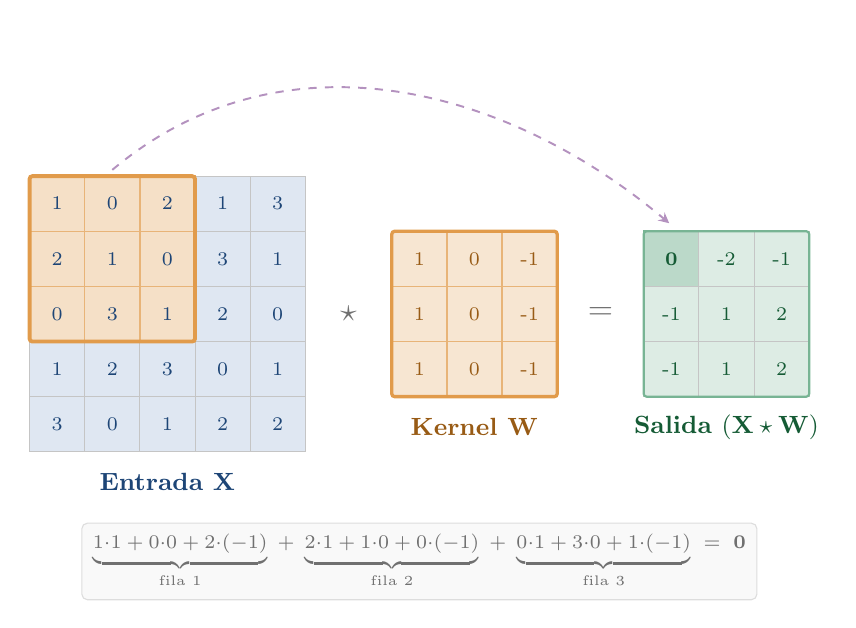
\begin{tikzpicture}[
    cell/.style={minimum size=0.7cm, inner sep=0pt, outer sep=0pt,
                 draw=gdlgray!50, line width=0.3pt},
    inputcell/.style={cell, fill=gdlblue!15},
    kernelhighlight/.style={cell, fill=gdlorange!25, draw=gdlorange!60,
                            line width=0.5pt},
    kernelcell/.style={cell, fill=gdlorange!20, draw=gdlorange!60,
                       line width=0.5pt},
    outputcell/.style={cell, fill=gdlgreen!15, draw=gdlgray!50},
    outputhighlight/.style={cell, fill=gdlgreen!30, draw=gdlgreen!60,
                            line width=0.6pt},
    lbl/.style={font=\small\bfseries},
]

\def\cs{0.7} % cell size

% ================================================================
% INPUT GRID (5x5)
% ================================================================
\def\ix{0}
\def\iy{0}

% Draw all 5x5 input cells
\foreach \r [count=\ri from 0] in {
  {1, 0, 2, 1, 3},
  {2, 1, 0, 3, 1},
  {0, 3, 1, 2, 0},
  {1, 2, 3, 0, 1},
  {3, 0, 1, 2, 2}} {
  \foreach \val [count=\ci from 0] in \r {
    \pgfmathsetmacro{\px}{\ix + \ci*\cs + \cs/2}
    \pgfmathsetmacro{\py}{\iy + (4-\ri)*\cs + \cs/2}
    \node[inputcell] at (\px, \py)
      {\scriptsize\color{gdlblue!70!black}\val};
  }
}

% Overlay: highlight the 3x3 kernel window (rows 0--2, cols 0--2)
\foreach \r [count=\ri from 0] in {
  {1, 0, 2},
  {2, 1, 0},
  {0, 3, 1}} {
  \foreach \val [count=\ci from 0] in \r {
    \pgfmathsetmacro{\px}{\ix + \ci*\cs + \cs/2}
    \pgfmathsetmacro{\py}{\iy + (4-\ri)*\cs + \cs/2}
    \node[kernelhighlight] at (\px, \py)
      {\scriptsize\color{gdlblue!70!black}\val};
  }
}

% Thick border around the kernel window on the input
\draw[gdlorange!80, line width=1.4pt, rounded corners=1pt]
  (\ix, \iy + 2*\cs) rectangle ++(3*\cs, 3*\cs);

% Input label (below grid, with extra spacing)
\node[lbl, text=gdlblue!70!black]
  at (\ix + 2.5*\cs, \iy - 0.55*\cs) {Entrada $\mathbf{X}$};

% ================================================================
% STAR OPERATOR
% ================================================================
\pgfmathsetmacro{\starx}{\ix + 5*\cs + 0.55}
\pgfmathsetmacro{\stary}{\iy + 2.5*\cs}
\node[font=\large, text=gdlgray!80!black] at (\starx, \stary) {$\star$};

% ================================================================
% KERNEL GRID (3x3) -- vertically centred with input
% ================================================================
\pgfmathsetmacro{\kx}{\starx + 0.55}
\pgfmathsetmacro{\ky}{\stary - 1.5*\cs}

\foreach \r [count=\ri from 0] in {
  {1, 0, -1},
  {1, 0, -1},
  {1, 0, -1}} {
  \foreach \val [count=\ci from 0] in \r {
    \pgfmathsetmacro{\px}{\kx + \ci*\cs + \cs/2}
    \pgfmathsetmacro{\py}{\ky + (2-\ri)*\cs + \cs/2}
    \node[kernelcell] at (\px, \py)
      {\scriptsize\color{gdlorange!70!black}\val};
  }
}

\draw[gdlorange!80, line width=1.2pt, rounded corners=1pt]
  (\kx, \ky) rectangle ++(3*\cs, 3*\cs);

\node[lbl, text=gdlorange!70!black]
  at (\kx + 1.5*\cs, \ky - 0.55*\cs) {Kernel $\mathbf{W}$};

% ================================================================
% EQUALS SIGN
% ================================================================
\pgfmathsetmacro{\eqx}{\kx + 3*\cs + 0.55}
\node[font=\large, text=gdlgray!80!black] at (\eqx, \stary) {$=$};

% ================================================================
% OUTPUT GRID (3x3) -- vertically centred with input
% ================================================================
\pgfmathsetmacro{\ox}{\eqx + 0.55}
\pgfmathsetmacro{\oy}{\ky}

\foreach \r [count=\ri from 0] in {
  {0, -2, -1},
  {-1, 1, 2},
  {-1, 1, 2}} {
  \foreach \val [count=\ci from 0] in \r {
    \pgfmathsetmacro{\px}{\ox + \ci*\cs + \cs/2}
    \pgfmathsetmacro{\py}{\oy + (2-\ri)*\cs + \cs/2}
    \ifnum\ri=0
      \ifnum\ci=0
        \node[outputhighlight] at (\px, \py)
          {\scriptsize\bfseries\color{gdlgreen!70!black}\val};
      \else
        \node[outputcell] at (\px, \py)
          {\scriptsize\color{gdlgreen!70!black}\val};
      \fi
    \else
      \node[outputcell] at (\px, \py)
        {\scriptsize\color{gdlgreen!70!black}\val};
    \fi
  }
}

\draw[gdlgreen!60, line width=0.8pt, rounded corners=1pt]
  (\ox, \oy) rectangle ++(3*\cs, 3*\cs);

\node[lbl, text=gdlgreen!70!black]
  at (\ox + 1.5*\cs, \oy - 0.55*\cs) {Salida $(\mathbf{X} \star \mathbf{W})$};

% ================================================================
% DASHED ARROW: kernel window on input --> highlighted output cell
% Start from top-centre of the kernel border, end at top of output cell
% ================================================================
\pgfmathsetmacro{\arcsrcx}{\ix + 1.5*\cs}          % horizontal centre of kernel window
\pgfmathsetmacro{\arcsrcy}{\iy + 5*\cs + 0.08}     % just above top of kernel border
\pgfmathsetmacro{\arctgtx}{\ox + 0.5*\cs}           % centre of highlighted output cell
\pgfmathsetmacro{\arctgty}{\oy + 3*\cs + 0.08}      % just above top of output grid

\draw[gdlpurple!55, dashed, line width=0.7pt, -stealth, shorten >=1pt]
  (\arcsrcx, \arcsrcy)
  to[out=40, in=140] (\arctgtx, \arctgty);

% ================================================================
% COMPUTATION DETAIL (below everything, with clear separation)
% ================================================================
\pgfmathsetmacro{\figcentrex}{(\ix + \ox + 3*\cs) / 2}
\pgfmathsetmacro{\compy}{\ky - 1.6}

\node[anchor=north, align=left, font=\scriptsize, text=gdlgray!80!black,
      inner sep=4pt, rounded corners=2pt,
      fill=gdlgray!5, draw=gdlgray!30, line width=0.4pt]
  at (\figcentrex, \compy) {%
    $\underbrace{1{\cdot}1 + 0{\cdot}0 + 2{\cdot}({-}1)}_{\text{fila 1}}
     \;+\;
     \underbrace{2{\cdot}1 + 1{\cdot}0 + 0{\cdot}({-}1)}_{\text{fila 2}}
     \;+\;
     \underbrace{0{\cdot}1 + 3{\cdot}0 + 1{\cdot}({-}1)}_{\text{fila 3}}
     \;=\; \mathbf{0}$};

\end{tikzpicture}
\end{document}
